\subsection{YOLO (v1)}
\begin{frame}{}
    \LARGE Object Detection: \textbf{YOLO (v1)}
\end{frame}

\begin{frame}{YOLO - Overview}
\only<1>{
\begin{figure}
\centering
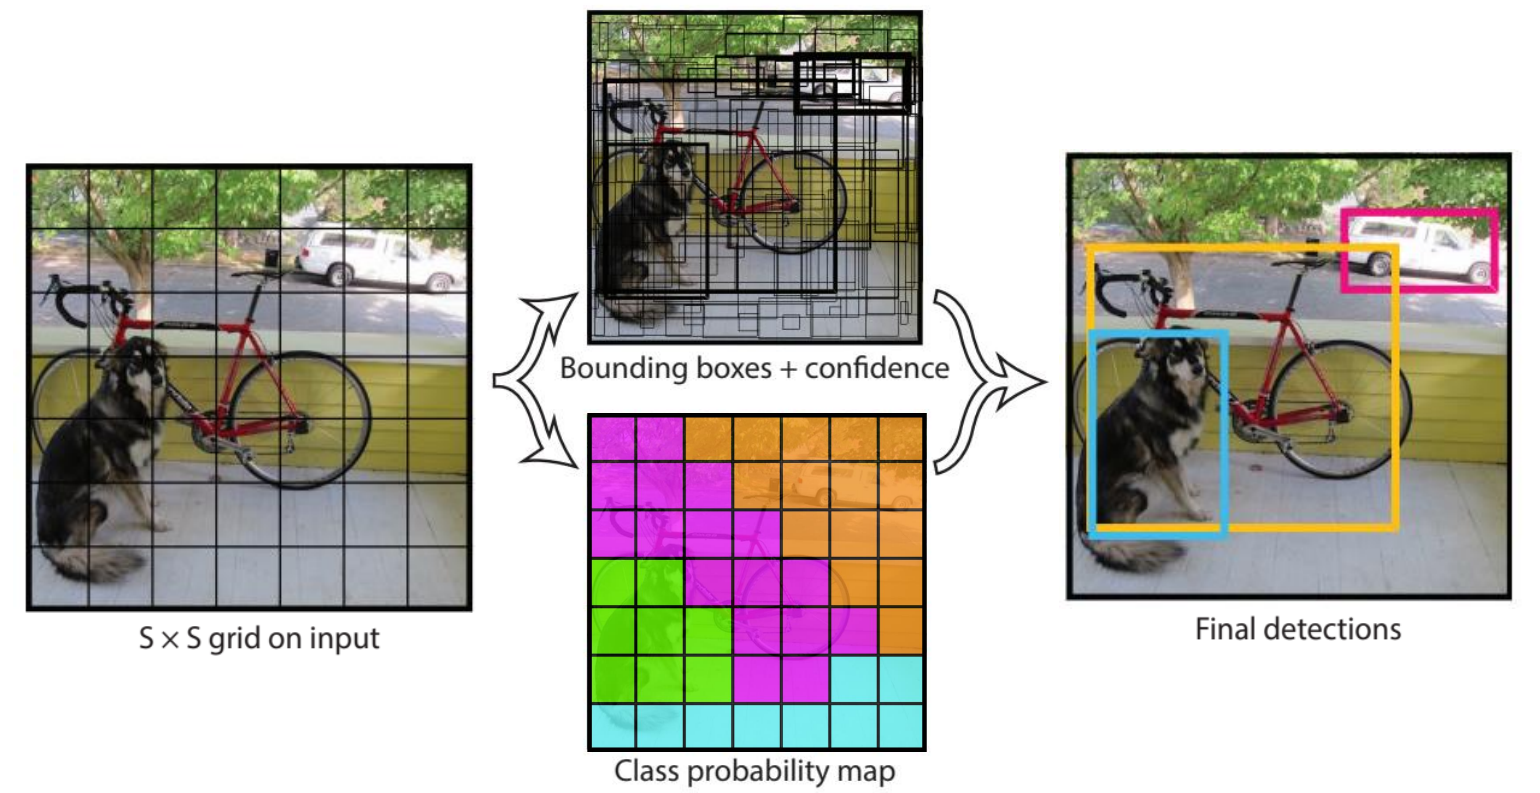
\includegraphics[width=1.0\textwidth,height=0.85\textheight,keepaspectratio]{images/object-detect/yolo_2.png}
\caption*{\tiny Source: WAIC DL4CV, ``Object Detection and Segmentation'' (Yariv, 2022), sl. 6; image: Redmon et al., CVPR 2016}
\end{figure}
}

\only<2>{
\begin{figure}
\centering
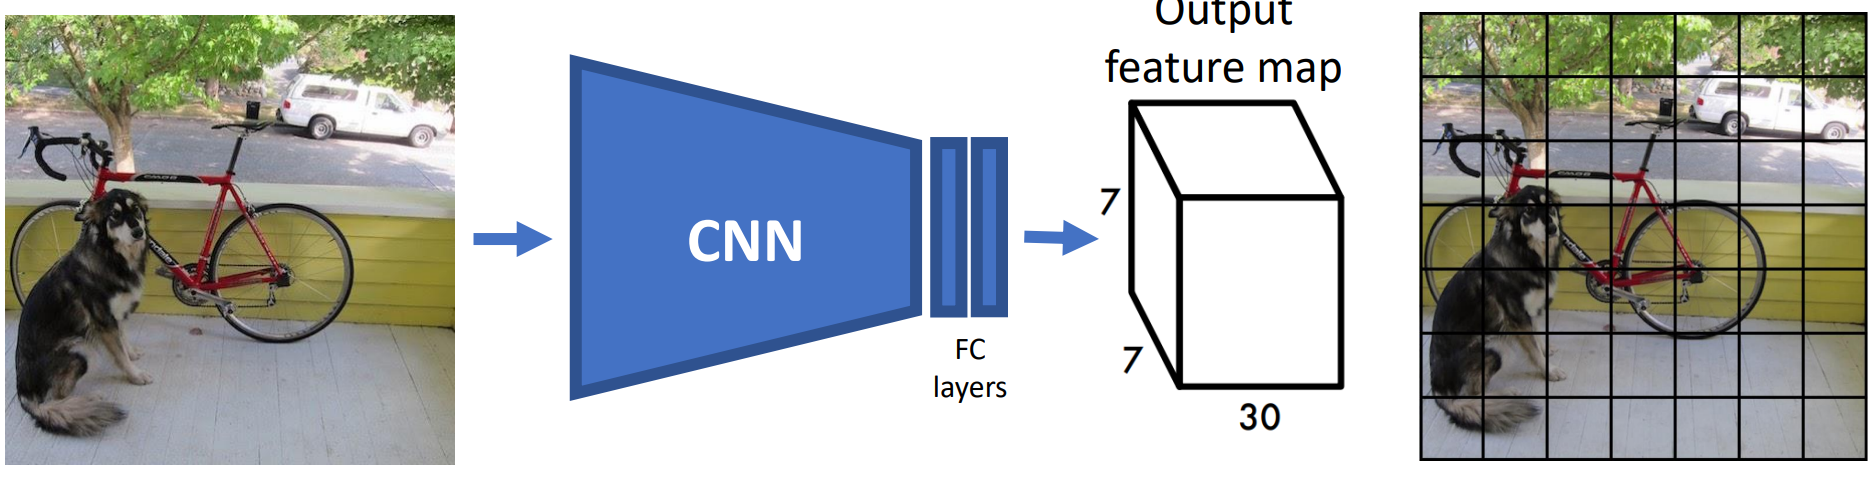
\includegraphics[width=1.0\textwidth,height=0.85\textheight,keepaspectratio]{images/object-detect/yolo_3.png}
\caption*{\tiny Source: WAIC DL4CV, ``Object Detection and Segmentation'' (Yariv, 2022), sl. 7; image: Redmon et al., CVPR 2016}
\end{figure}
}
\only<3>{
\begin{figure}
\centering
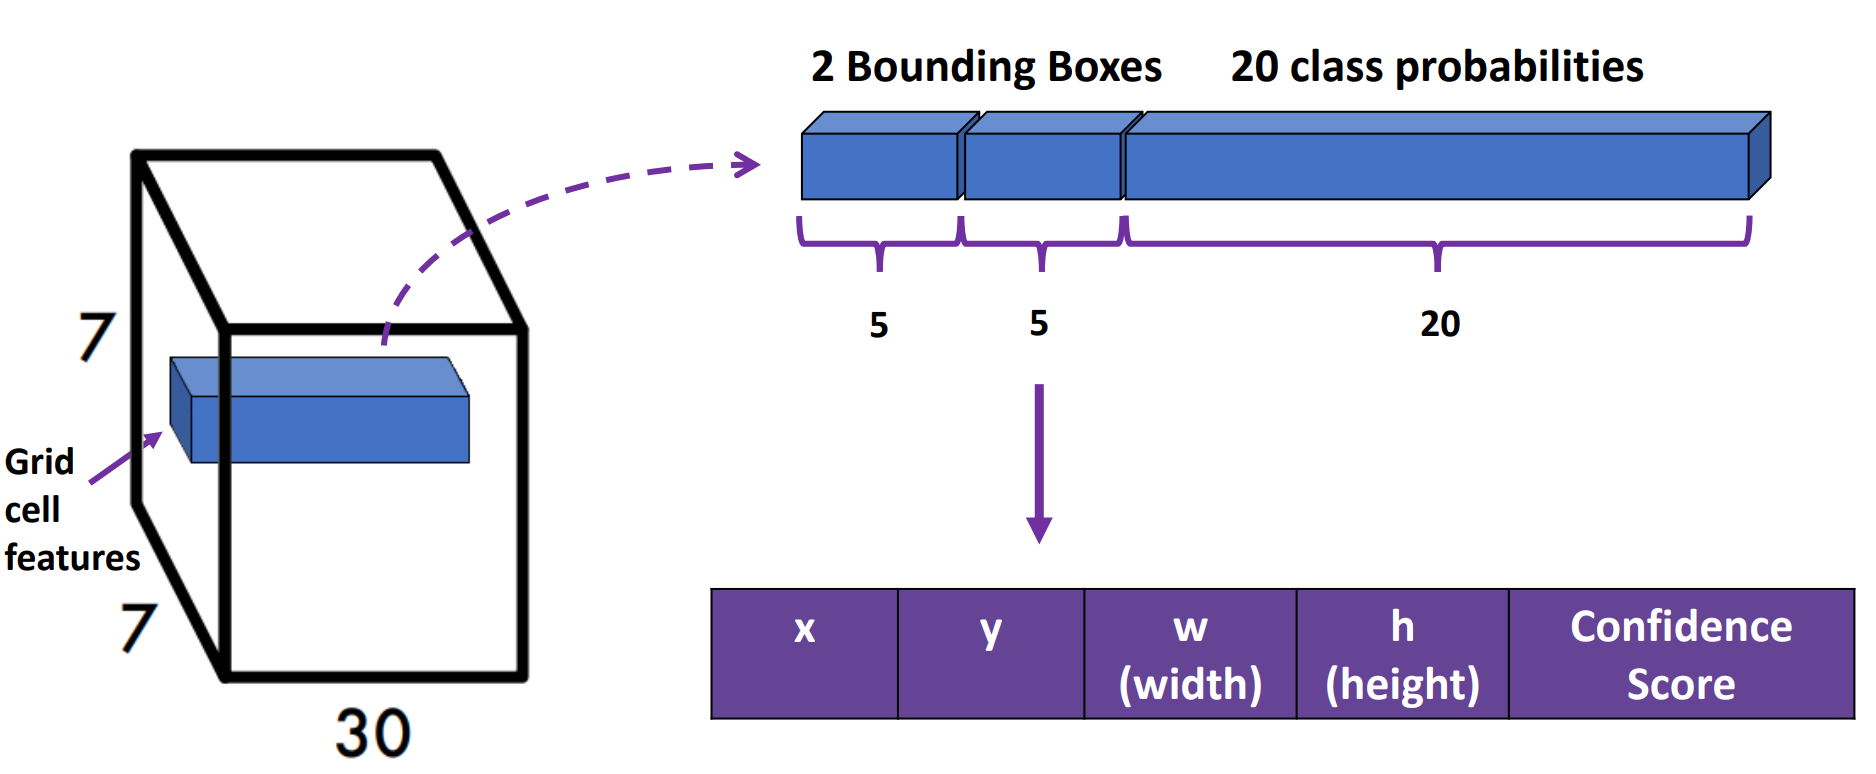
\includegraphics[width=1.0\textwidth,height=0.85\textheight,keepaspectratio]{images/object-detect/yolo_4.png}
\caption*{\tiny Source: WAIC DL4CV, ``Object Detection and Segmentation'' (Yariv, 2022), sl. 12; image: Redmon et al., CVPR 2016}
\end{figure}
}
    
\end{frame}

\begin{frame}{YOLO}
\begin{columns}
    \begin{column}{0.5\textwidth}
    \onslide<2->{Each cell predicts}
    \begin{itemize}
        \item<3-> $B=2$ bounding boxes $(x,y,w,h) + $ confidence score
        \item<4-> $C=20$ class probabilities
        \vspace{1cm}
        \item<8-> Apply Non-Maximum Suppression
    \end{itemize}
    \end{column}
    
    \begin{column}{0.5\textwidth}
    \only<-2>{
    \begin{figure}
    \centering
    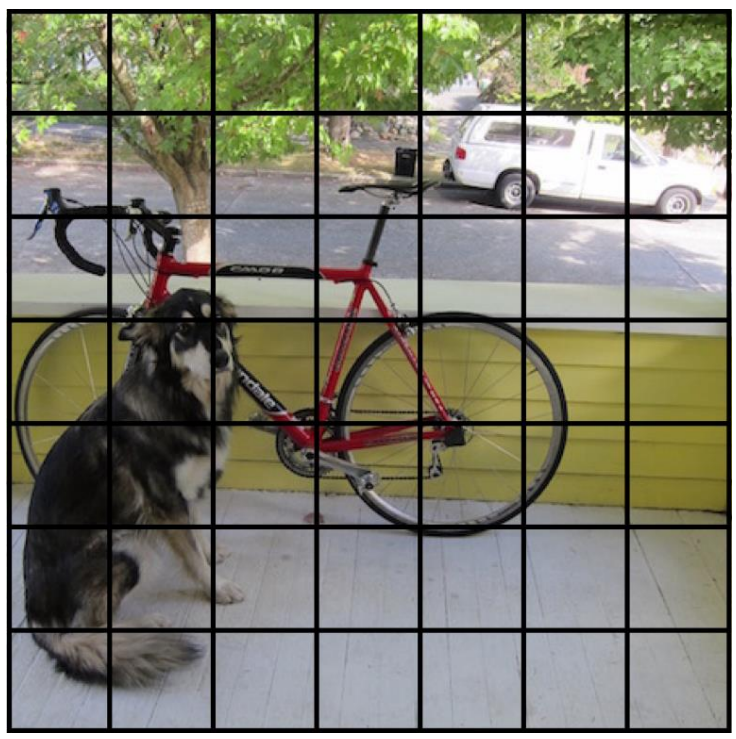
\includegraphics[width=1.0\textwidth,height=0.75\textheight,keepaspectratio]{images/object-detect/yolo_5.png}
    \caption*{\tiny Source: WAIC DL4CV, ``Object Detection and Segmentation'' (Yariv, 2022), sl. 8; image: Redmon et al., CVPR 2016}
    \end{figure}
    }

    \only<3-4>{
    \begin{figure}
    \centering
    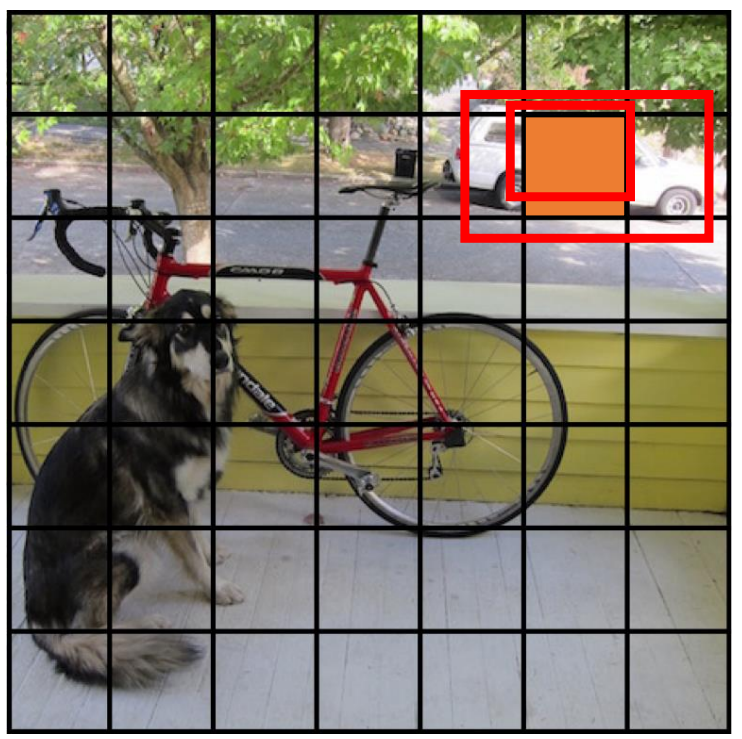
\includegraphics[width=1.0\textwidth,height=0.75\textheight,keepaspectratio]{images/object-detect/yolo_6.png}
    \caption*{\tiny Source: WAIC DL4CV, ``Object Detection and Segmentation'' (Yariv, 2022), sl. 10; image: Redmon et al., CVPR 2016}
    \end{figure}
    }

    \only<5>{
    \begin{figure}
    \centering
    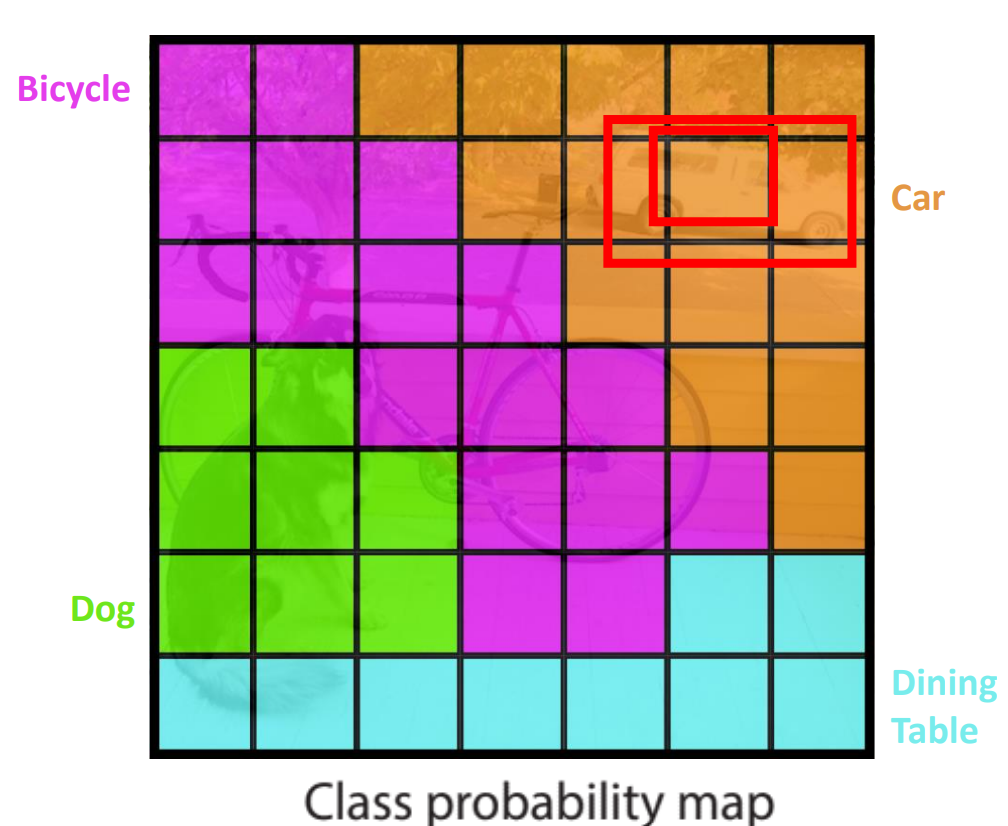
\includegraphics[width=1.0\textwidth,height=0.75\textheight,keepaspectratio]{images/object-detect/yolo_7.png}
    \caption*{\tiny Source: WAIC DL4CV, ``Object Detection and Segmentation'' (Yariv, 2022), sl. 11; image: Redmon et al., CVPR 2016}
    \end{figure}
    }

    \only<6>{
    \begin{figure}
    \centering
    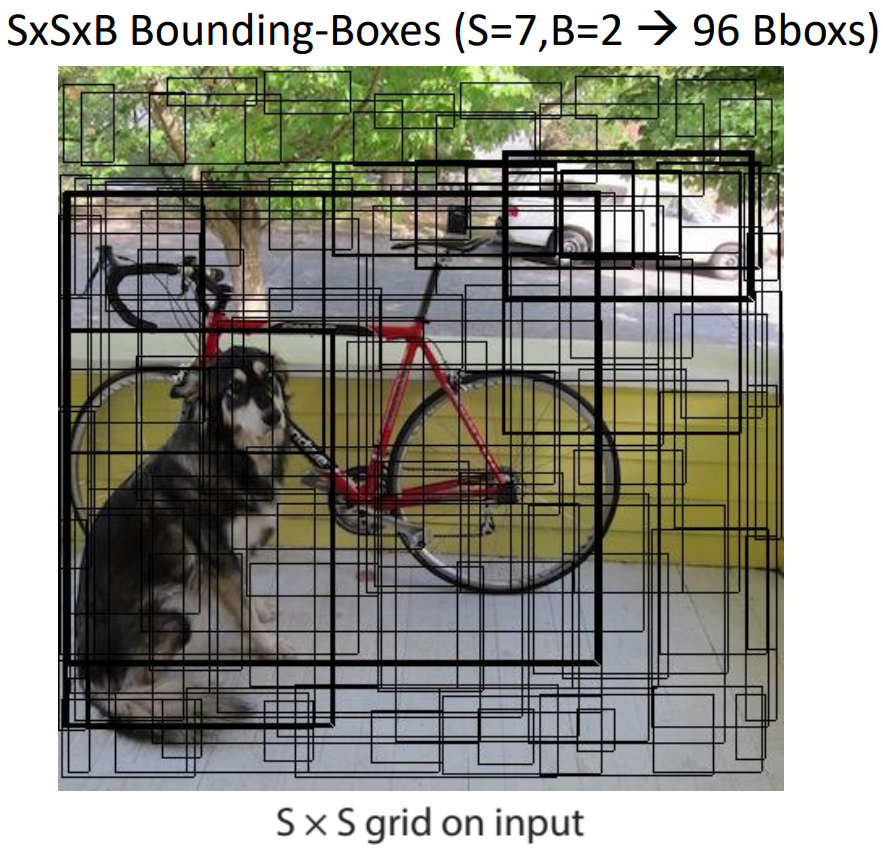
\includegraphics[width=1.0\textwidth,height=0.75\textheight,keepaspectratio]{images/object-detect/yolo_8.png}
    \caption*{\tiny Source: WAIC DL4CV, ``Object Detection and Segmentation'' (Yariv, 2022), sl. 13; image: Redmon et al., CVPR 2016}
    \end{figure}
    }

    \only<7>{
    \begin{figure}
    \centering
    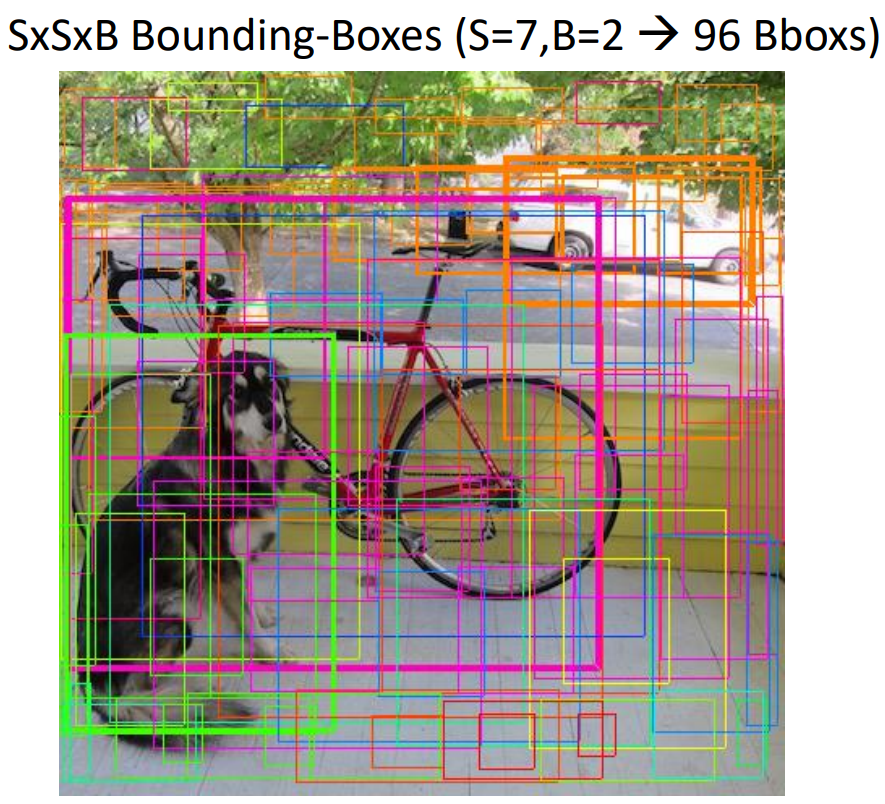
\includegraphics[width=1.0\textwidth,height=0.75\textheight,keepaspectratio]{images/object-detect/yolo_9.png}
    \caption*{\tiny Source: WAIC DL4CV, ``Object Detection and Segmentation'' (Yariv, 2022), sl. 14; image: Redmon et al., CVPR 2016}
    \end{figure}
    }

    \only<8>{
    \begin{figure}
    \centering
    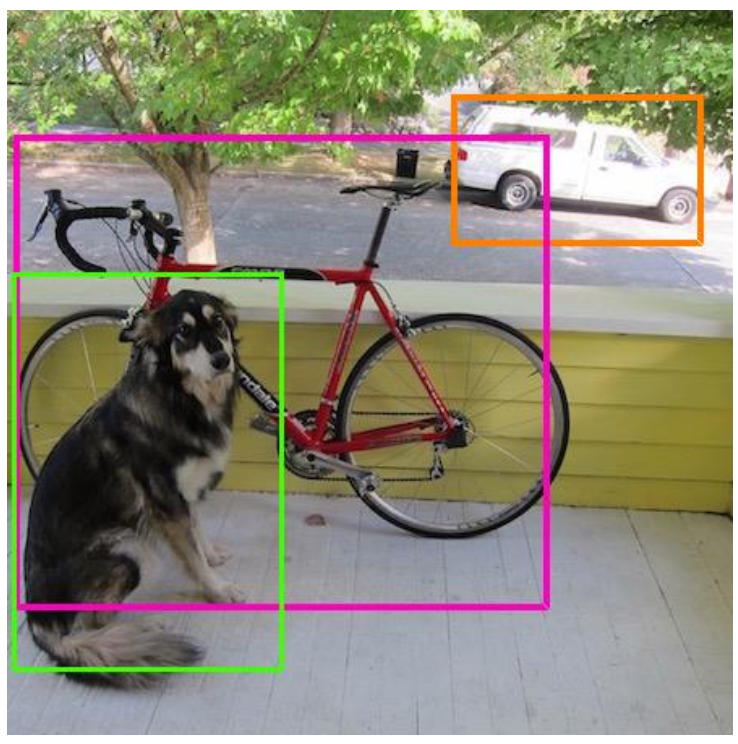
\includegraphics[width=1.0\textwidth,height=0.75\textheight,keepaspectratio]{images/object-detect/yolo_10.png}
    \caption*{\tiny Source: WAIC DL4CV, ``Object Detection and Segmentation'' (Yariv, 2022), sl. 15; image: Redmon et al., CVPR 2016}
    \end{figure}
    }
        
    \end{column}
\end{columns}
    
\end{frame}

\begin{frame}{YOLO - Loss Function}
    \begin{figure}
    \centering
    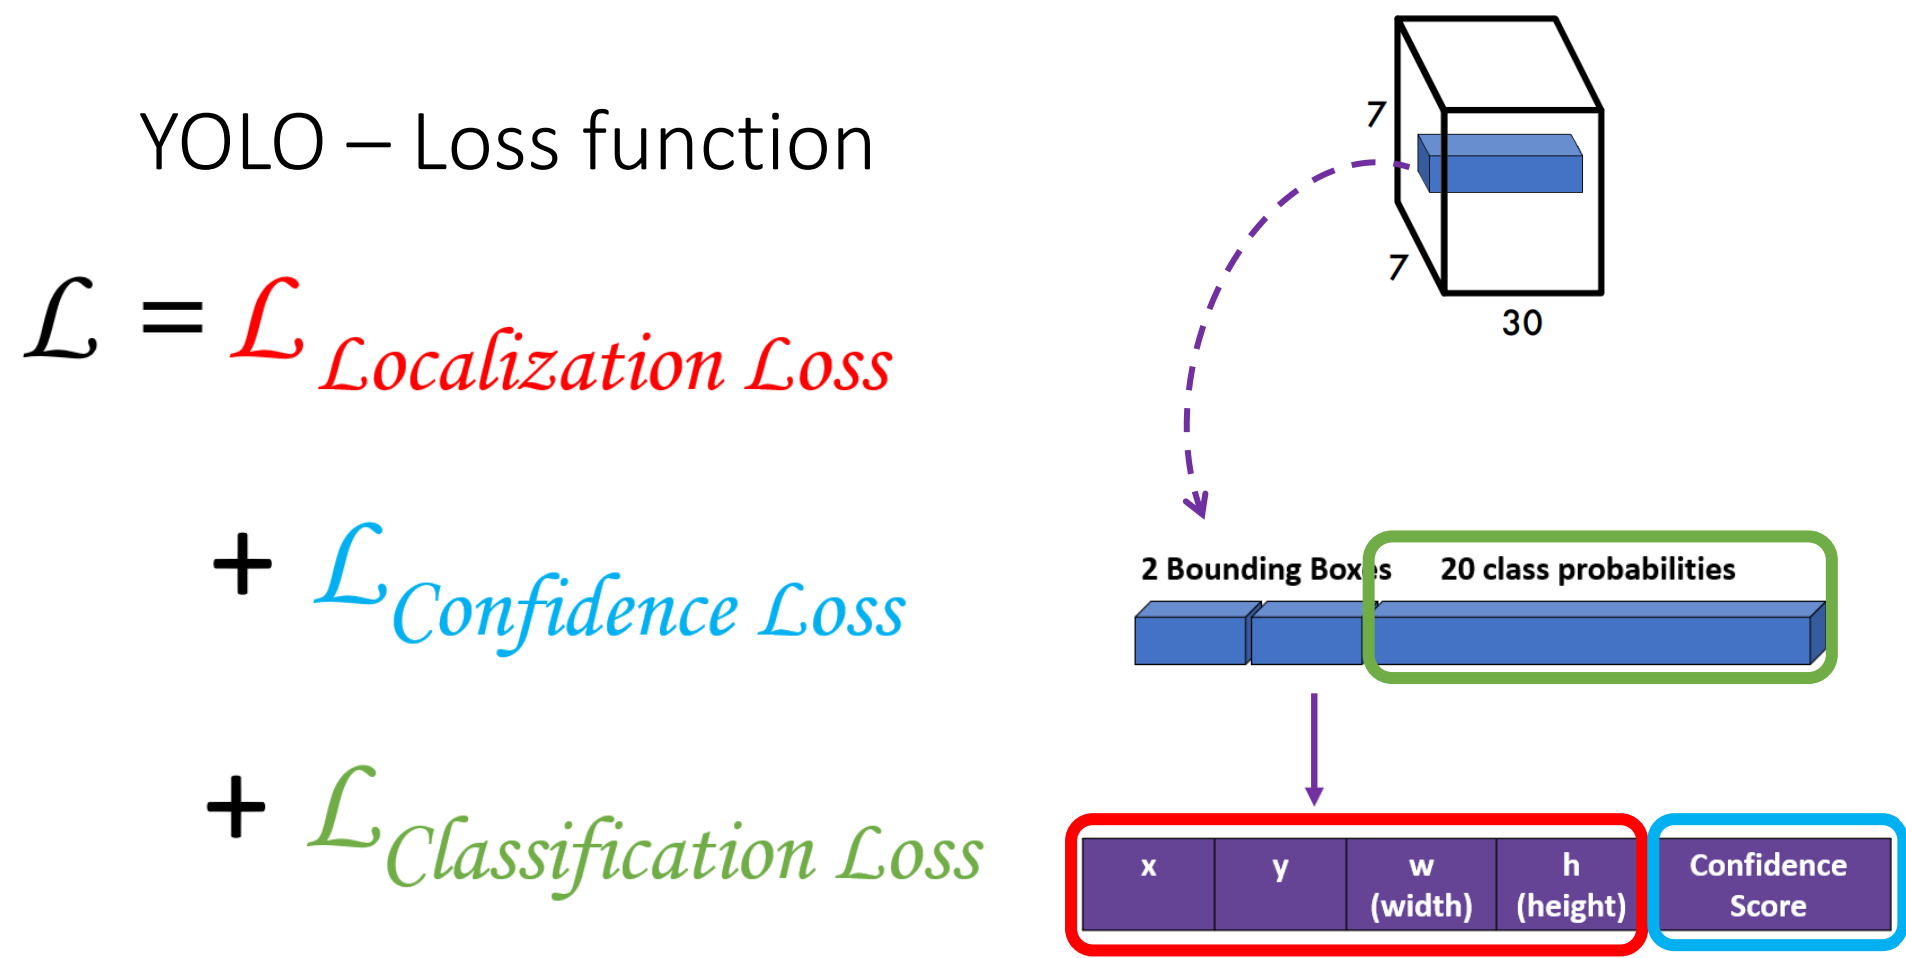
\includegraphics[width=1.0\textwidth,height=0.82\textheight,keepaspectratio]{images/object-detect/yolo_11.png}
    \caption*{\tiny Source: WAIC DL4CV, ``Object Detection and Segmentation'' (Yariv, 2022), sl. 19; image: Redmon et al., CVPR 2016}
    \end{figure}
\end{frame}



\begin{frame}{YOLO - Benefits}
\begin{columns}
    \begin{column}{0.6\textwidth}
    \begin{itemize}
        \item Fast. Good for real-time processing
        \item End-to-end training
    \end{itemize}
    \begin{figure}
    \centering
    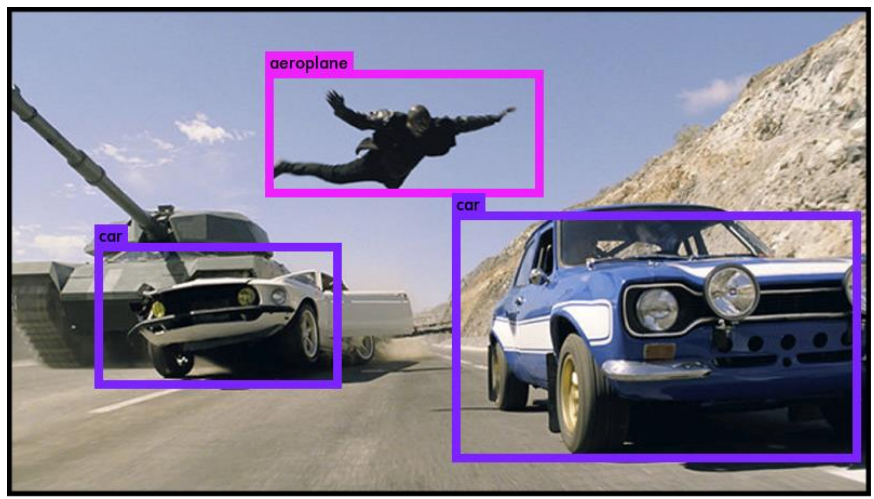
\includegraphics[width=1.0\textwidth,height=0.78\textheight,keepaspectratio]{images/object-detect/yolo_12.png}
    \caption*{\tiny Source: WAIC DL4CV, ``Object Detection and Segmentation'' (Yariv, 2022), sl. 29; image: Redmon et al., CVPR 2016}
    \end{figure}
    
    \end{column}
    
    \begin{column}{0.4\textwidth}
    \begin{figure}
    \centering
    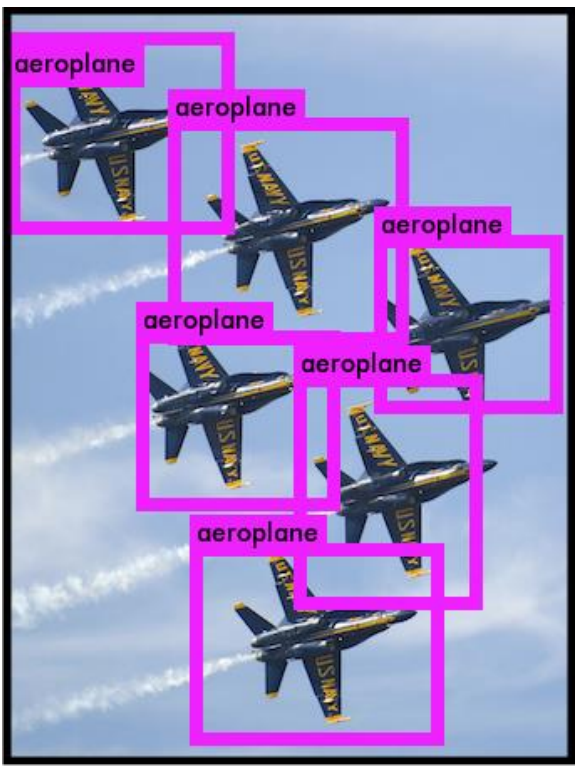
\includegraphics[width=1.0\textwidth,height=0.78\textheight,keepaspectratio]{images/object-detect/yolo_13.png}
    \caption*{\tiny Source: WAIC DL4CV, ``Object Detection and Segmentation'' (Yariv, 2022), sl. 29; image: Redmon et al., CVPR 2016}
    \end{figure}
        
    \end{column}
\end{columns}
    
\end{frame}

\begin{frame}{YOLO - Limitations}
\begin{columns}
    \begin{column}{0.5\textwidth}
    \begin{itemize}
        \item<2-> Difficult to detect small objects
        \item<2-> Coarse predictions
        \item<3-> Fixed input size
        \item<4-> A grid cell can predict only one class
        \vspace{0.5cm}
        \onslide<5->{
        \item \textcolor{red}{Solutions:}
        \begin{itemize}
            \item Remove fc layers!
            \item Predict class per bbox (not per cell)
        \end{itemize}
        }
    \end{itemize}
    \end{column}
    
    \begin{column}{0.5\textwidth}
    \only<-2>{
    \begin{figure}
    \centering
    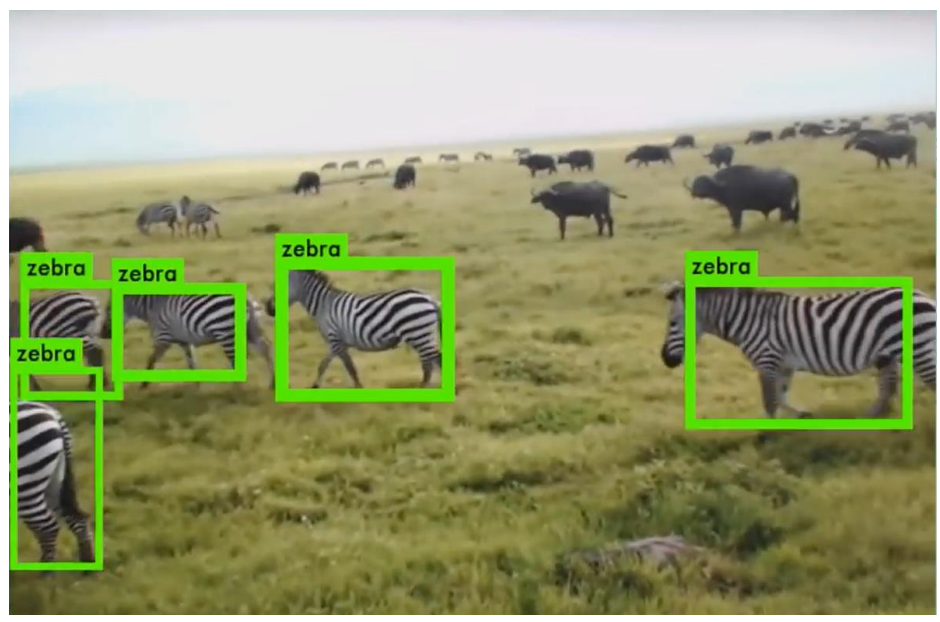
\includegraphics[width=1.0\textwidth,height=1.0\textheight,keepaspectratio]{images/object-detect/yolo_14.png}
    \caption*{\tiny Source: WAIC DL4CV, ``Object Detection and Segmentation'' (Yariv, 2022), sl. 30; image: \url{https://pjreddie.com/darknet/yolov1/}}
    \end{figure}
    }

    \only<3>{
    \begin{figure}
    \centering
    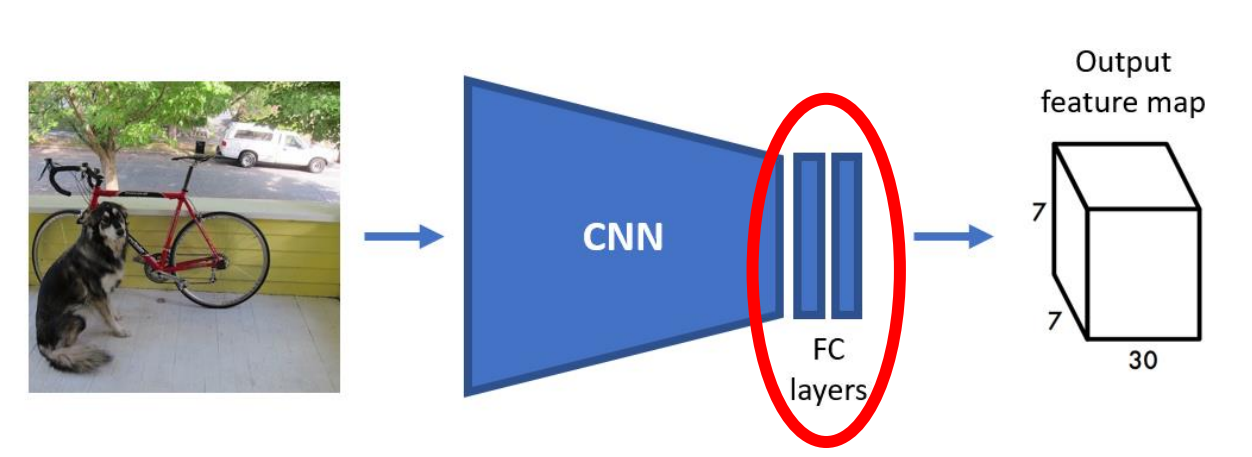
\includegraphics[width=1.0\textwidth,height=1.0\textheight,keepaspectratio]{images/object-detect/yolo_15.png}
    \caption*{\tiny Source: WAIC DL4CV, ``Object Detection and Segmentation'' (Yariv, 2022), sl. 32; image: Redmon et al., CVPR 2016}
    \end{figure}
    }

    \only<4->{
    \begin{figure}
    \centering
    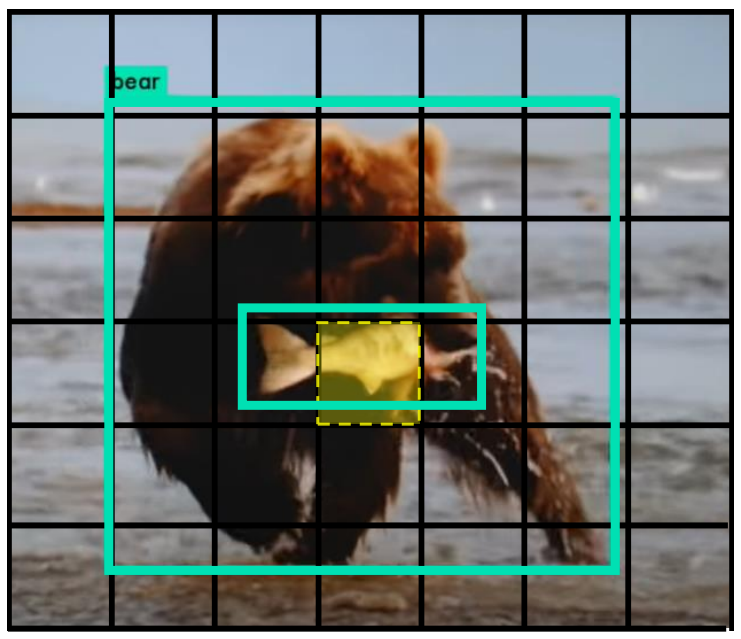
\includegraphics[width=1.0\textwidth,height=1.0\textheight,keepaspectratio]{images/object-detect/yolo_16.png}
    \caption*{\tiny Source: WAIC DL4CV, ``Object Detection and Segmentation'' (Yariv, 2022), sl. 33; image: \url{https://pjreddie.com/darknet/yolov1/}}
    \end{figure}
    }
        
    \end{column}
\end{columns}
\end{frame}